\subsection{Analisis Hasil Pengujian}

\subsubsection{Analisis Hasil Pengujian Sistem}

Secara umum, hasil pengujian sistem menunjukkan bahwa sistem pencarian berbasis semantik memberikan hasil yang lebih relevan dibandingkan dengan sistem pencarian berbasis teks. Selain itu, sistem pencarian berbasis semantik juga dapat menghasilkan relevansi yang baik untuk masukan berupa query bahasa alami dan kata kunci. Sedangkan sistem pencarian berbasis teks hanya dapat menerima masukan berupa kata kunci untuk mendapatkan hasil pencarian yang relevan. Hal ini menunjukkan fleksibilitas sistem pencarian berbasis semantik untuk menghasilkan hasil yang relevan berdasarkan jenis masukan yang berbeda.

Selain itu, hasil untuk sistem pencarian berbasis semantik pada iterasi perbaikan menunjukkan peningkatan presisi yang signifikan dibandingkan dengan iterasi awal. Hal ini menunjukkan bahwa proses iterasi perbaikan, yaitu perubahan prompt, format data, konteks Source Code yang lengkap, dan penambahan deskripsi semantik, memberikan dampak positif yang terlihat terhadap relevansi hasil pencarian.

\subsubsection{Analisis Skalabilitas Sistem}

Skalabilitas sistem dapat dilihat dari aspek teknis sistem pada bagian \ref{subsec:teknis-sistem}. Untuk menilai skalabilitas sistem, diperlukan referensi jumlah data yang ada pada blockchain saat ini. Berdasarkan data dari Etherscan yang diambil pada 31 Juli 2025, jumlah Smart Contracts yang ada pada blockchain Ethereum pada network mainnet adalah 79.598.826 Smart Contracts dengan 790.354 diantaranya adalah Verified Smart Contracts. Data lengkap terkait jumlah data Smart Contracts dapat dilihat pada Gambar \ref{image:etherscan-smart-contracts}. Fokus dari sistem ini adalah pada Verified Smart Contracts, karena fokus sistem ini adalah untuk memberikan hasil pencarian yang dapat dimanfaatkan untuk digunakan ulang. Smart Contracts yang tidak terverifikasi tidak memiliki seringkali merupakan kontrak yang berbahaya, kosong, atau duplikat, sehingga tidak dianjurkan untuk digunakan ulang.

\begin{figure}[ht]
	\centering
	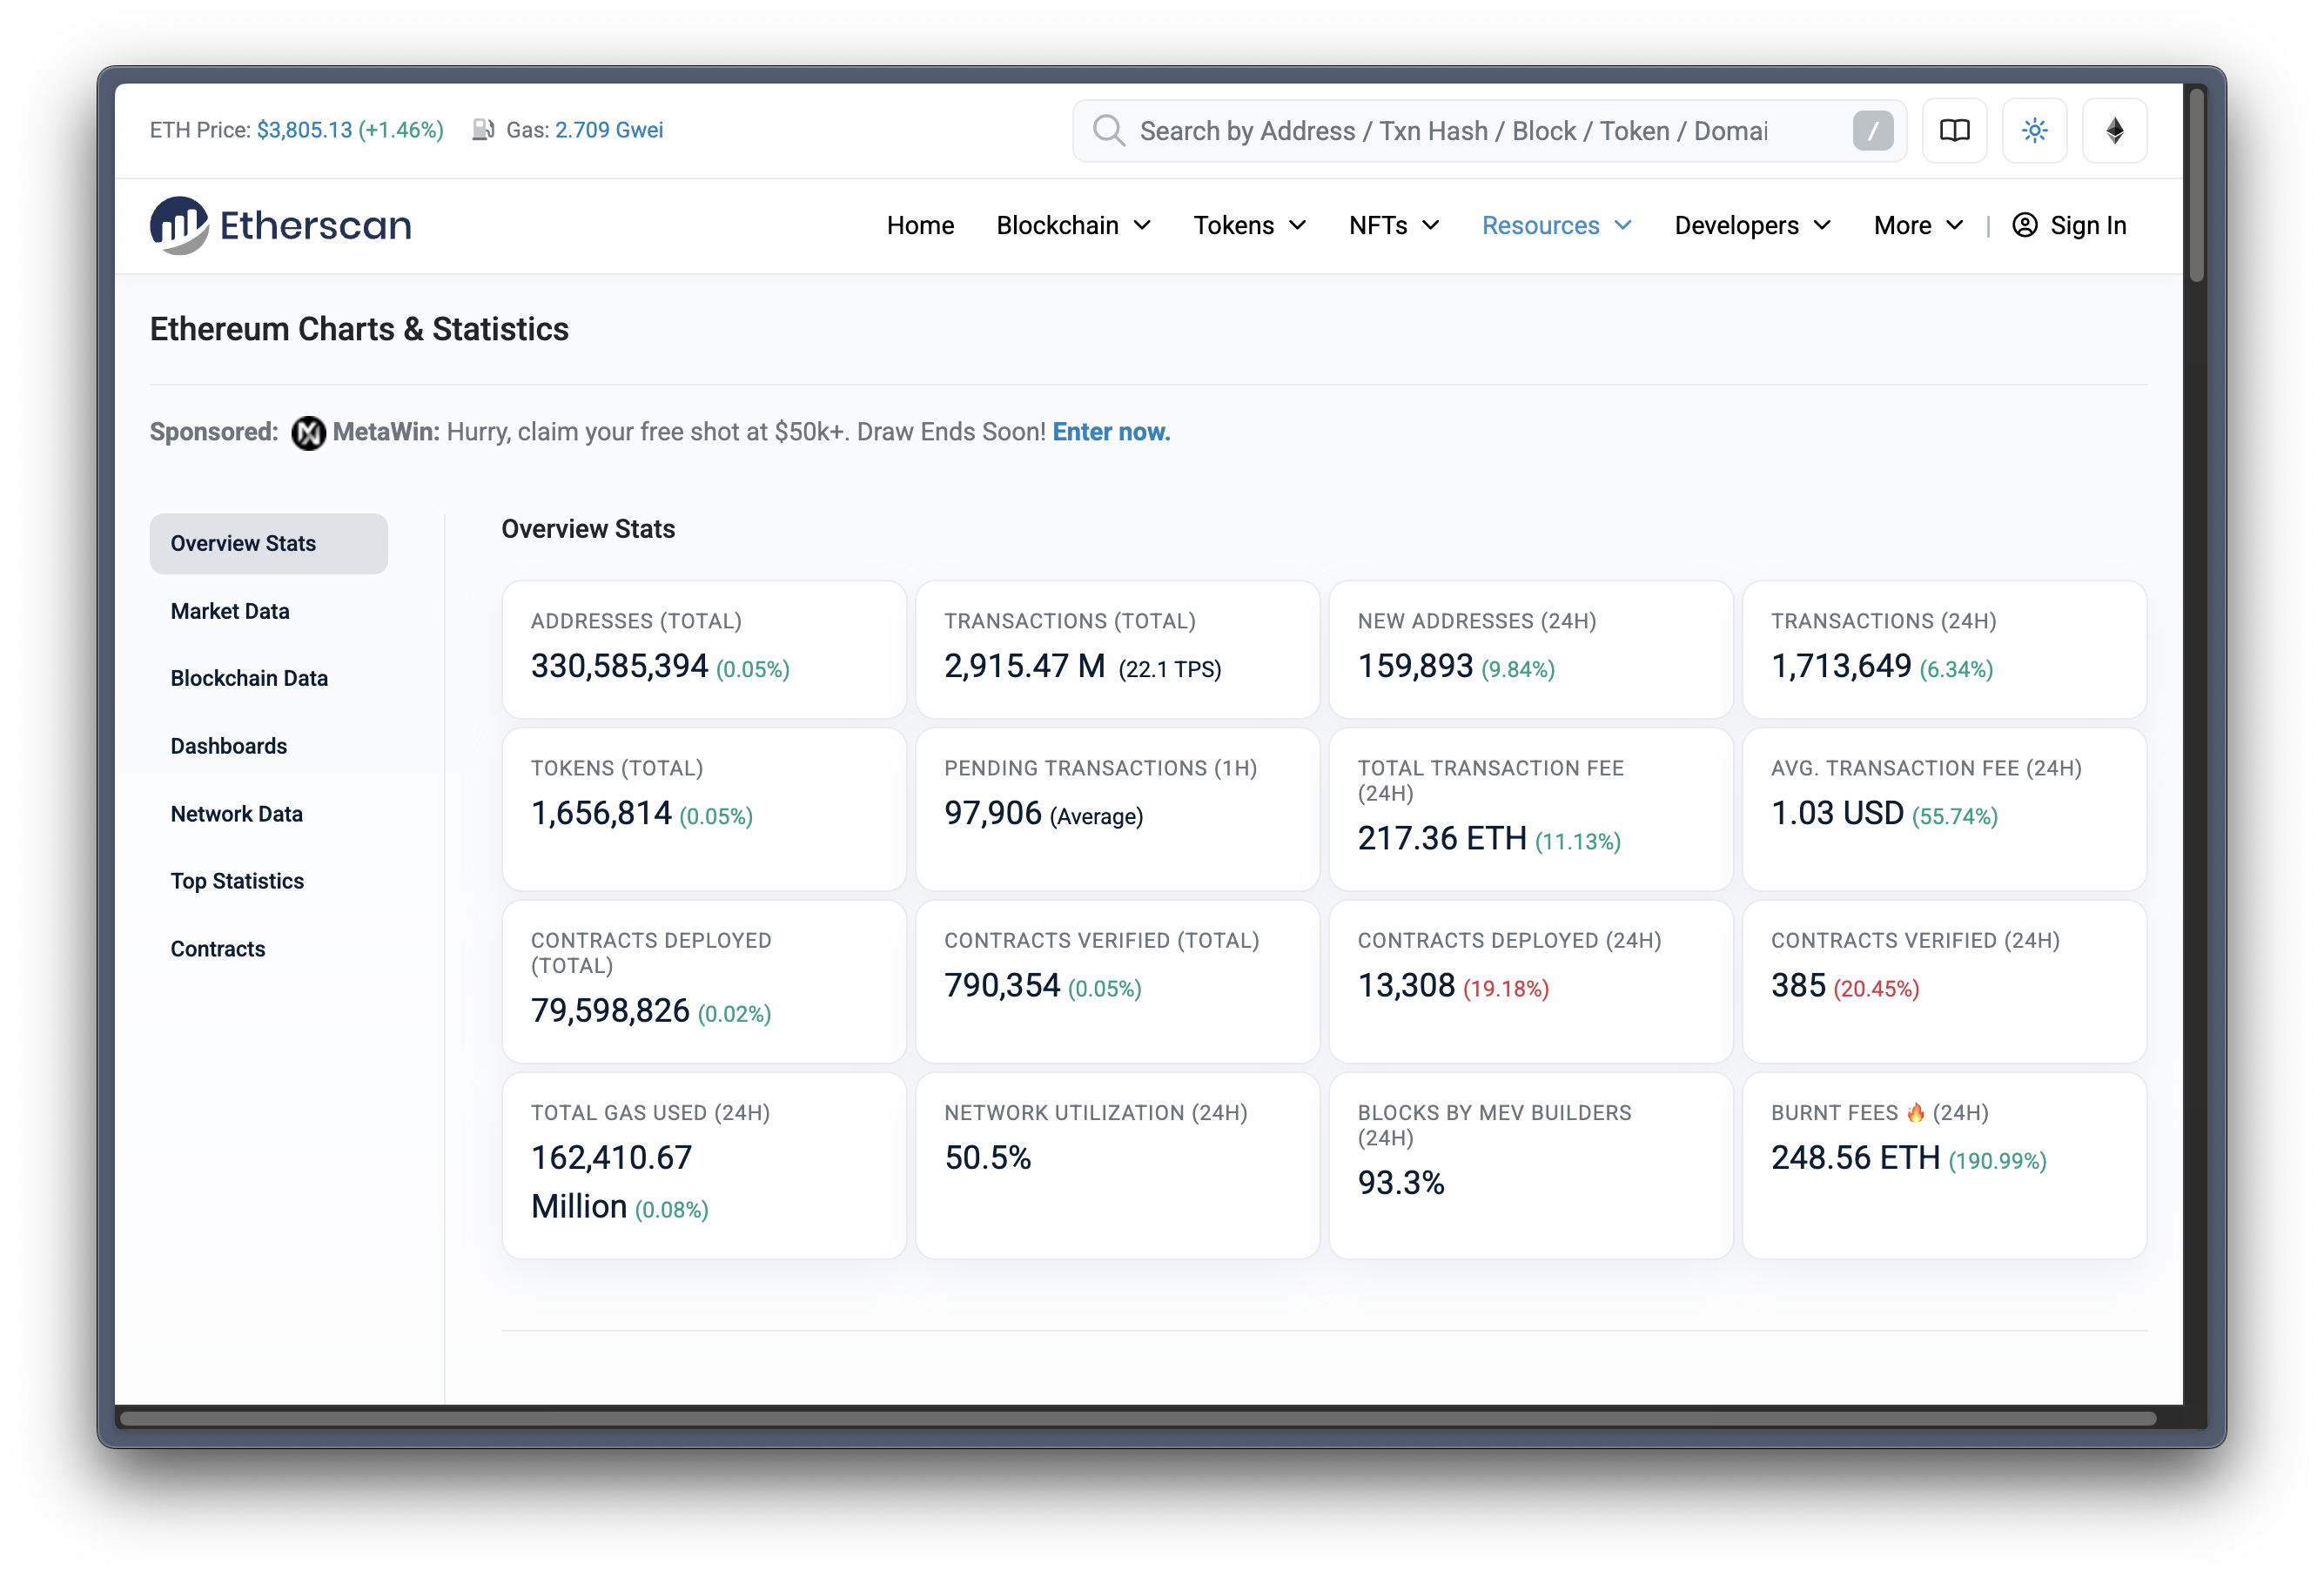
\includegraphics[width=1\textwidth]{resources/chapter-4/smart-contracts.png}
	\caption{Statistik Ethereum Mainnet}
	\label{image:etherscan-smart-contracts}
\end{figure}

Berdasarkan data yang didapatkan saat melakukan proses enrichment, didapatkan \textit{baseline calculation}:

\begin{align*}
    \text{Biaya per Kontrak} &= \frac{\text{Total Biaya}}{\text{Kontrak Diproses}} \\
    &= \frac{C_{\text{total}}}{N} \\
    &= \frac{\$0,23}{118} \\
    &\approx \$0,00195 \text{ per contract}
\end{align*}

Waktu rata-rata yang per kontrak dapat diaproksimasi menggunakan P50:
\[
\text{Waktu rata-rata per Kontrak} \approx T_{\text{P50}} = 5,56 \text{ detik}
\]

Menggunakan kedua unit tersebut, dapat ditinjau dua analisis utama, yaitu analisis skalabilitas berdasarkan biaya dan waktu.

\subsubsubsection{Analisis Skalabilitas Biaya}

Analisis akan menggunakan dua lingkup, yaitu lingkup Verified Smart Contracts, yang akan lebih mungkin untuk digunakan ulang dan semua Smart Contracts. Berikut merupakan perhitungan yang digunakan:

\begin{align*}
	C_{\text{estimated, verified}} &= N_{\text{verified}} \times C_{\text{unit}} \\
	&= 790.354 \text{ contracts} \times \$0,00195/\text{contract} \\
	&\approx \$1.541
\end{align*}

Biaya yang akan dikeluarkan untuk menganalisis seluruh Verified Smart Contracts sekitar \$1.500. Biaya ini dapat diterima secara skalabilitas karena hanya perlu dilakukan satu kali analisis dan hasil akan disimpan secara persisten sehingga tidak perlu melakukan analisis pada kontrak yang sama berulang kali.

Selanjutnya, untuk perhitungan dari biaya semua Smart Contracts:

\begin{align*}
	C_{\text{estimated, total}} &= N_{\text{total}} \times C_{\text{unit}} \\
	&= 79.598.826 \text{ contracts} \times \$0,00195/\text{contract} \\
	&\approx \$155.218
\end{align*}

Dibutuhkan biaya sebesar sekitar \$150.000 untuk menganalisis seluruh Smart Contracts yang ada pada blockchain. Hal ini menunjukkan bahwa percobaan memproses seluruh data Smart Contracts pada blockchain, termasuk jutaan kontrak kosong, simpel, atau duplikat, akan menjadi sangat mahal.

\subsubsubsection{Analisis Skalabilitas Waktu}

Waktu yang dibutuhkan akan bergantung pada kapabilitas sistem untuk memproses data secara paralel. Untuk kepentingan analisis, akan dihitung dua skenario, yaitu sekuensial atau tidak paralel, dan paralel dengan 100 proses. Berikut merupakan perhitungan yang digunakan:

\begin{align*}
	T_{\text{sequential, total}} &= N_{\text{total}} \times T_{\text{avg}} \\
	&= 79.598.826 \text{ contracts} \times 5,56 \text{ \text{s}/\text{contract}} \\
	&= 442.569.471,56 \text{s} \\
	T_{\text{sequential, verified}} &= N_{\text{verified}} \times T_{\text{avg}} \\
	&= 790.354 \text{ contracts} \times 5,56 \text{ \text{s}/\text{contract}} \\
	&= 4.394.368,24 \text{s}
\end{align*}

Waktu yang dibutuhkan untuk memproses seluruh kontrak adalah sekitar 14 tahun dan untuk seluruh Verified Smart Contracts adalah sekitar 51 hari. Hal ini menunjukkan bahwa pemrosesan sekuensial akan tidak \textit{scalable}. Tetapi, pemrosesan satu data dengan data yang lain merupakan proses yang \textit{mutually exclusive}, sehingga dapat diproses secara paralel dengan tidak terbatas. Secara teori, skalabilitas waktu dari sistem dapat terjaga dengan baik. Berikut merupakan perhitungan untuk pemrosesan paralel dengan 100 proses:

\begin{align*}
    T_{\text{parallel, total}} &= \frac{T_{\text{sequential, total}}}{P} \\
    &= \frac{14 \text{ hari}}{100 \text{ proses}} \\
	&\approx 51 \text{ hari} \\
    T_{\text{parallel, verified}} &= \frac{T_{\text{sequential, verified}}}{P} \\
    &= \frac{51 \text{ hari}}{100 \text{ proses}} \\
	&\approx 12,2 \text{ jam}
\end{align*}

Perhitungan berikut menunjukkan bahwa dengan pemrosesan paralel, waktu yang dibutuhkan untuk memproses seluruh kontrak dapat dikurangi secara signifikan. Hal yang harus diperhatikan adalah P99 sistem yaitu 9,41 detik, yang bernilai hampir dua kali dari P50, sehingga dapat membuat waktu pemrosesan lebih panjang dibandingkan perkiraan yang dihitung.

\subsubsubsection{Analisis Skalabilitas Penyimpanan}

Data utama yang disimpan pada sistem ini adalah data Smart Contracts, terutama Source Code dari Verified Smart Contracts. Data yang digunakan oleh sistem, yaitu sebanyak 118 data Smart Contracts, memiliki ukuran total 2,8 MB. Referensi yang dapat digunakan untuk memperkirakan ukuran data Smart Contracts jika seluruh Verified Smart Contracts diproses adalah data dari Smart Contract Sanctuary Ethereum. Repositori ini berisikan 344.250 Smart Contracts dengan ukuran total 28 GB. Sehingga perkiraan ukuran data Smart Contracts jika seluruh Verified Smart Contracts diproses adalah sekitar 60 GB. Hal ini menunjukkan bahwa masih memungkinkan untuk sistem dapat mengakomodasi penyimpanan seluruh data Verified Smart Contracts.

\subsubsubsection{Analisis Latensi Pencarian}

Latensi pencarian pada sistem ini dapat dibagi menjadi dua, yaitu latensi pencarian pada Dgraph dan waktu pemrosesan Natural Language Query menjadi embeddings. Data latensi pencarian pada Dgraph dapat dilihat pada Gambar \ref{image:latency-dgraph}. Latensi pencarian pada Dgraph memiliki P99 sebesar 134,51 ms dan P50 sebesar 76,03 ms. Hal ini menunjukkan bahwa Dgraph dapat memberikan hasil pencarian dengan cepat. Data waktu pemrosesan Natural Language Query menjadi embeddings dapat dilihat pada Gambar \ref{image:latency-embeddings}. Waktu pemrosesan Natural Language Query menjadi embeddings memiliki P99 sebesar 2,5 detik dan P50 sebesar 73,82 ms. Hal ini menunjukkan bahwa waktu pemrosesan Natural Language Query menjadi embeddings masih dapat diterima, meskipun lebih lama dibandingkan dengan latensi pencarian pada Dgraph. Lonjakan waktu pemrosesan yang terlihat pada data disebabkan oleh lonjakan load pada CPU yang digunakan untuk menjalankan model embeddings, sehingga menyebabkan waktu pemrosesan menjadi lebih lama. Hal ini tidak akan dibahas lebih lanjut karena berada di luar lingkup topik, sehingga fokus analisis hanya pada latensi pencarian pada Dgraph.

\begin{figure}[ht]
	\centering
	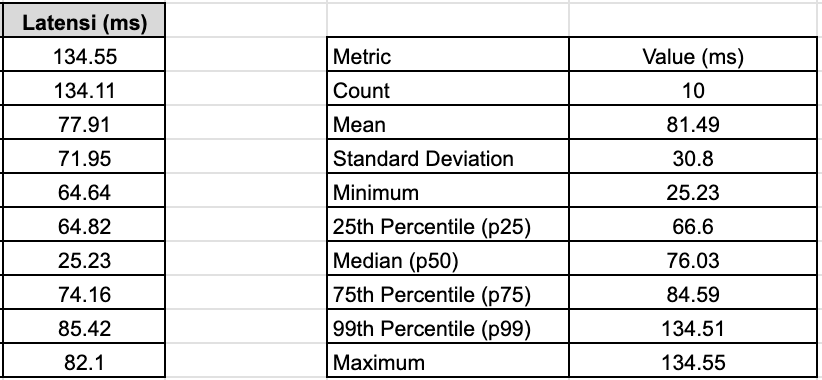
\includegraphics[width=0.75\textwidth]{resources/chapter-4/data-latensi.png}
	\caption{Statistik Latensi Pencarian pada Dgraph}
	\label{image:latency-dgraph}
\end{figure}

\begin{figure}[ht]
	\centering
	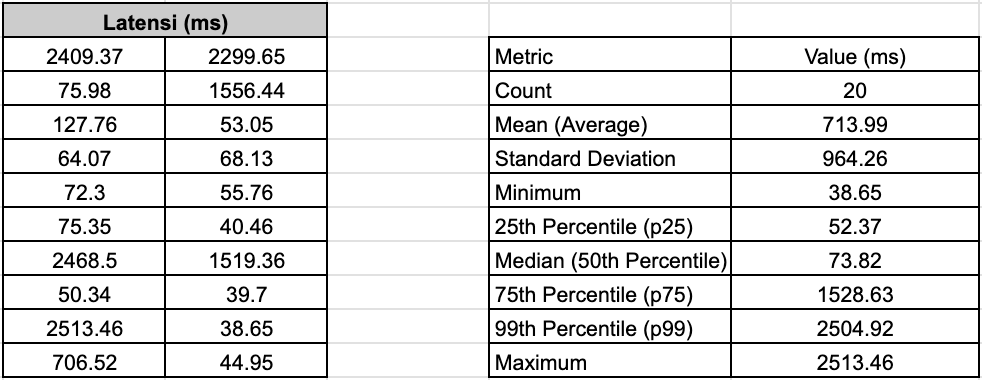
\includegraphics[width=0.75\textwidth]{resources/chapter-4/data-latensi-embeddings.png}
	\caption{Statistik Waktu Pemrosesan Natural Language Query menjadi Embeddings}
	\label{image:latency-embeddings}
\end{figure}

Secara skalabilitas, latensi pencarian pada Dgraph terbukti cukup baik saat diuji dengan 250 GB data pada pengujian yang dilakukan oleh tim pengembang Dgraph \parencite{hypermode_performance}. Dimana latensi pencarian tidak pernah melebihi 5 detik untuk seluruh pengujian yang dilakukan, bahkan untuk beban 1000 koneksi paralel dengan 2 core. Pengujian yang dilakukan oleh \cite{ashwin2016distributed} juga menjamin dari skalabilitas Dgraph. Pada lingkup Verified Smart Contracts, latensi pencarian pada Dgraph diperkirakan akan lebih baik dibandingkan dengan pengujian yang dilakukan oleh tim Hypermode, karena jumlah data yang lebih sedikit dan juga Dgraph sudah dioptimasi untuk menangani data yang lebih besar dengan skalabilitas horizontal sistem yang tinggi dengan arsitekturnya.

\subsubsubsection{Hasil Analisis Skalabilitas}

Sistem dapat dinilai cukup \textit{scalable} secara waktu, tetapi butuh perhatian khusus pada aspek biaya. Aspek biaya ini dapat menjadi lebih \textit{scalable} seiring berjalannya waktu dengan harga token yang semakin berkurang, atau dapat menggunakan model yang lebih murah dengan \textit{tradeoff} kualitas hasil enrichment, selain itu, dapat juga menggunakan model Open Source yang \textit{self-hosted} untuk meminimalisir biaya.

Secara sistem, fokus analisis hanya pada proses enrichment karena proses retrieval sepenuhnya ditangani oleh Dgraph, dengan metrik retrieval yang sudah dilakukan \textit{benchmark}, selain itu proses \textit{data loading} juga sepenuhnya ditangani oleh eth2dgraph dengan metrik yang tertera pada risetnya.
